\section{Results}

\subsection{Route agreement does not imply performance safety}

Before hidden drift, the operational network and twin use the indirect route and measure 0.153 ms and 0.184 ms mean RTT. With 30 ms per-direction hidden delay, the candidate makes both environments select next hop \texttt{192.168.2.2} with metric 15. The twin reports 0.166 ms, but the operational network measures 66.274 ms: a 66.108 ms residual and a false-safe decision without route disagreement. Fig.~\ref{fig:rtt} shows the divergence as hidden delay increases.

\begin{figure}[t]
\centering
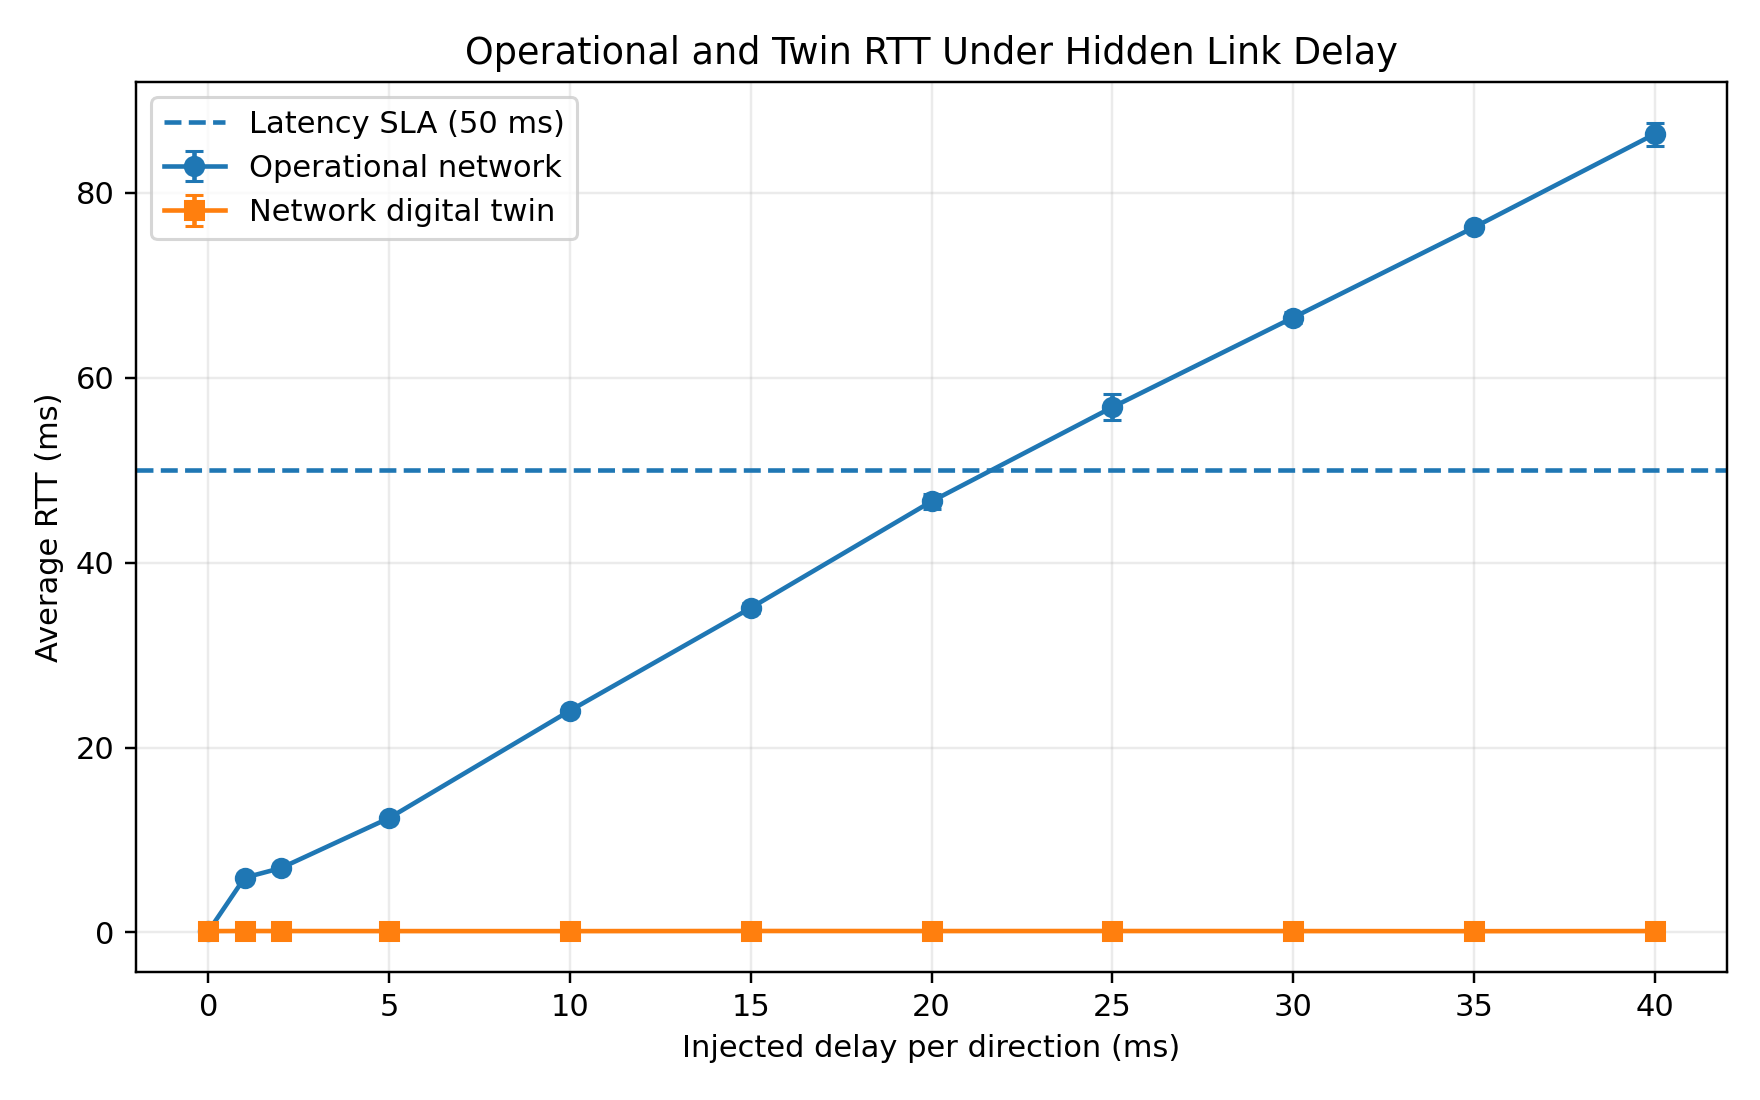
\includegraphics[width=\columnwidth]{figures/figure1_rtt_vs_delay.png}
\caption{Operational and twin RTT versus hidden candidate-link delay.}
\label{fig:rtt}
\end{figure}

\subsection{Residual-only gates are unsafe or vacuous}

Phase 4 shows why global residual history is insufficient in the tested mixed schedules. Direct, twin-only, and a fixed 10 ms margin accept all 186 candidates and each deploys 65 unsafe changes. The static residual quantile and rolling windows of 20 and 50 reject all candidates. A 10-observation rolling window accepts 16, including two unsafe candidates, and covers only 14/121 safe candidates (11.57\%). It also fails the cross-schedule utility criterion. Zero unsafe deployments under complete abstention is therefore not counted as successful safety.

\subsection{The sentinel restores useful discrimination}

Table~\ref{tab:outcomes} summarizes Phase 5. The frozen sentinel accepts 110/186 candidates, including 109/112 safe candidates, and admits one unsafe candidate. Relative to twin-only validation, unsafe deployments fall from 74 to one (98.65\% reduction) while safe-change coverage remains 97.32\%. The single unsafe accepted case is near the decision boundary: corrected prediction 48.922 ms, upper score 49.583 ms, and observed RTT 50.229 ms. The three safe rejections are likewise concentrated near the 20 ms per-direction regime.

Across validation, candidate-link correction reduces MAE from 38.154 ms to 0.745 ms and yields Pearson $r=0.9993$ with observed RTT (Fig.~\ref{fig:pred}). This indicates that most error in this controlled experiment is localized to the activated link.

\begin{figure}[t]
\centering
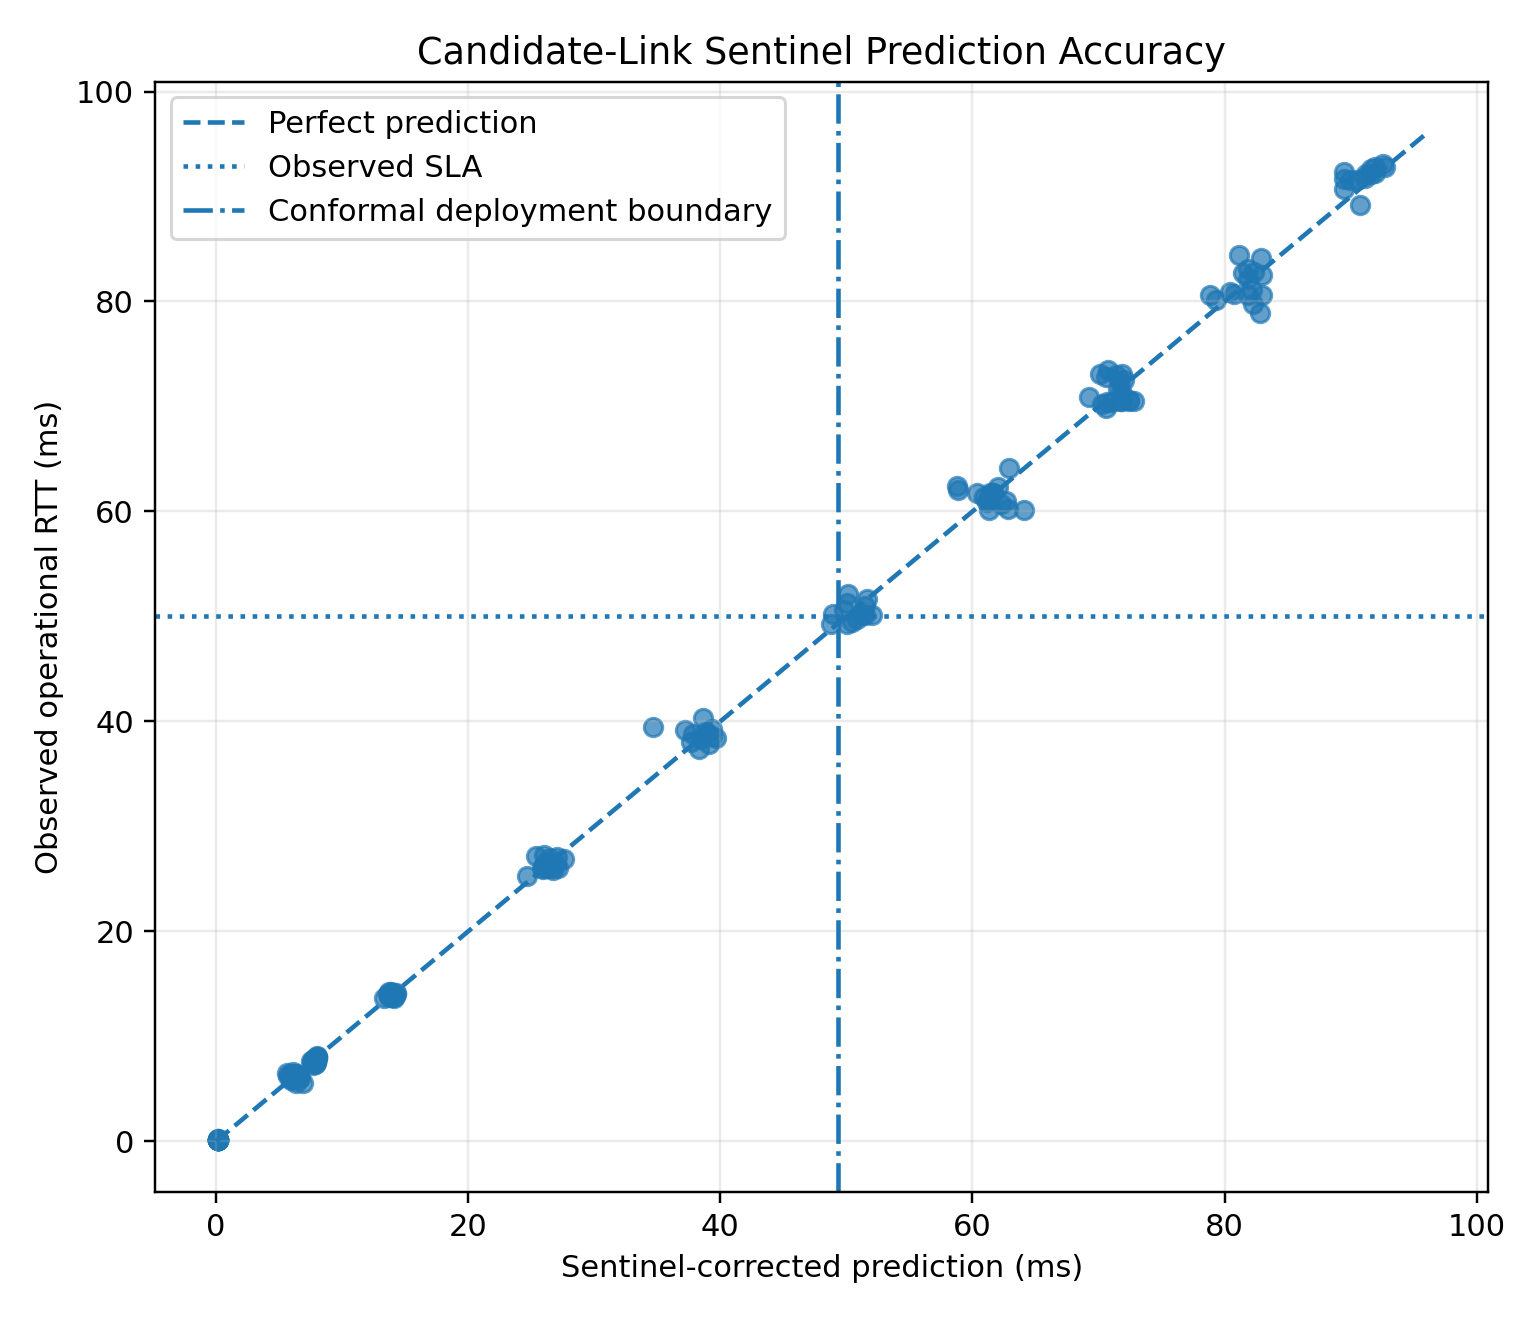
\includegraphics[width=\columnwidth]{figures/phase5_prediction_vs_observed.png}
\caption{Corrected prediction versus observed operational RTT during validation.}
\label{fig:pred}
\end{figure}

\subsection{Held-out evaluation and coverage failure}

On the 33-sample holdout, the frozen policy accepts all 19 safe candidates and rejects all 14 unsafe candidates. Thus no classification error is observed, but the 95\% Wilson interval for the unsafe rate among the 19 accepted changes is 0--16.82\%; the data do not establish zero underlying risk. The raw sentinel would accept one additional unsafe case (corrected 49.985 ms, observed 50.967 ms); the 0.661 ms margin moves its score to 50.646 ms and rejects it.

Prediction accuracy remains strong: holdout MAE drops from 40.917 ms for the uncorrected twin to 0.990 ms, RMSE is 1.440 ms, and Pearson $r=0.9991$. However, the one-sided upper score covers only 150/186 validation RTTs (80.65\%) and 20/33 holdout RTTs (60.61\%), not the nominal 95\%. Binary SLO classification and predictive-interval validity must therefore not be conflated. The supported claim is empirical deployment safety and utility in the tested regime, not distribution-free conformal coverage.

\begin{table*}[!t]
\caption{Phase 5 validation and holdout outcomes.}
\label{tab:outcomes}
\centering
\scriptsize
\begin{tabularx}{\textwidth}{l r r r r r r}
\toprule
Partition / policy & Samples & Accepted & Unsafe deployed & Safe accepted & Safe coverage & Unsafe/accepted\\
\midrule
Validation: Direct & 186 & 186 & 74 & 112 & 100.00\% & 39.78\%\\
Validation: Twin only & 186 & 186 & 74 & 112 & 100.00\% & 39.78\%\\
Validation: Raw sentinel & 186 & 111 & 2 & 109 & 97.32\% & 1.80\%\\
Validation: Frozen sentinel & 186 & 110 & 1 & 109 & 97.32\% & 0.91\%\\
Holdout: Frozen sentinel & 33 & 19 & 0 & 19 & 100.00\% & 0.00\%\\
\bottomrule
\end{tabularx}
\end{table*}
